
\chapter{Einleitung}

Dieses Kapitel soll den Leser auf den Inhalt der Arbeit 
aufmerksam machen, ihn mit der Aufgabestellung vertraut 
machen und "uber die Strukturierung und Zielsetzung der 
Arbeit Auskunft geben.


\section{Motivation}
Objekte werden in der heutigen Zeit immer mehr mit 
Elektronik und Intelligenz versehen. Die Leute wollen 
aufgrund dieser Entwicklung, dass Prozesse oder 
bestimmte Aufgaben ohne menschliches Eingreifen 
erledigt und miteinander vernetzt werden. Das System 
soll lediglich "uberwacht und die Ergebnisse zu 
bestimmten Zwecken benutzt werden.

Das Internet der Dinge (\ac{IoT}) wird dazu genutzt, um 
die Interaktion zwischen Menschen und vernetzten 
elektronischen Ger"aten zu vereinfachen. 


\section{Aufgabenstellung und Zielsetzung}
Man m"ochte Daten wie, den Energieverbrauch eines Hauses, 
die Bewegung eines Objekts oder die Temperatur eines Raums 
kennen und "uber lange Strecken (20 km) "ubertagen ohne 
hohe Kosten mit  geringem Energieverbrauch. Es gibt 
heutzutage Technologien, wie \ac{GSM}, Bluetooth oder Wi-Fi, 
die diese Arbeit erledigen k"onnen. Das Problem dabei 
ist, dass beim Nutzen von GSM hohe Lizenzkosten 
fallen k"onnen. Was Bluetooth und Wifi betrifft, ist 
ihre Reichweite sehr begrenzt. Dieses Ziel kann mithilfe 
der LoRa-Technologie erreicht werden, da sie diese 
Nachteile beseitigt.  

In dieser Abschlussarbeit soll ein Prototyp gebaut 
werden, der mithilfe der LoRa-Technologie Daten an 
einen Anwendungsserver sendet und von diesem Server Daten 
empf"angt. Anders gesagt, diese Bachelorarbeit 
besch"aftigt sich mit der Entwicklung eines vernetzten 
Systems bestehend aus einem 3D-Beschleuni-gungssensor, 
einem 3D-Gyroskop sowie einem Tem\-peratur- und 
Feuchtigkeitssensor. Die Sensoren messen Daten und 
"ubergeben diese an den STM32L475 Mikrocontroller.

Der Mikrocontroller soll die Daten verarbeiten und mithilfe eines 
LoRa-Moduls \cite{AT_Command} drahtlos an 
einen Server "ubertragen. Bevor die "Ubertragung 
erfolgt, muss das LoRa-Endger"at Zugang zu dem Netzwerk 
durch den Server bekommen. Nachdem das LoRa-Endger"at 
dem Netzwerk hinzugef"ugt wurde, k"onnen nun 
Informationen zwischen dem LoRa-Endger"at und dem 
Netzwerk-Server bis zu einem Anwendungsserver 
ausgetauscht werden. Abbildungen \ref{fig:LRWAN} und 
\ref{fig:LabcsmartLoRawan} geben einen "Uberblick "uber 
den Aufbau des gesamten Systems.

\vspace{2cm}
\begin{figure}[h]
	\centering
	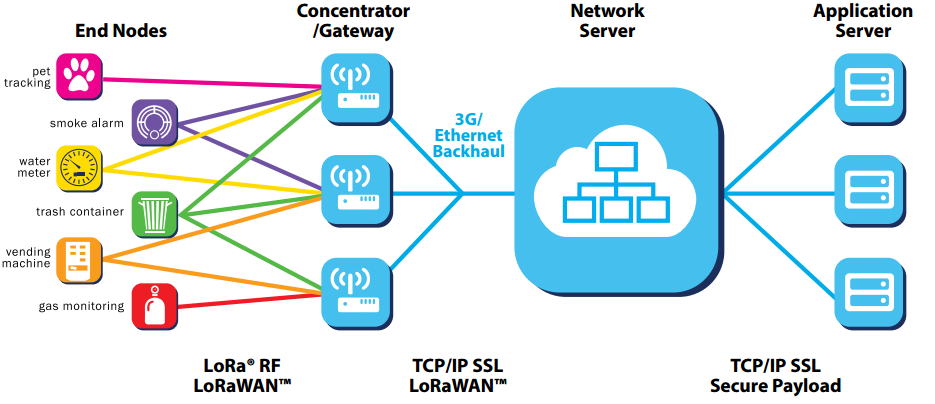
\includegraphics[width=15cm]{source/images/LoRaWAN_NET}
	\caption{Allgemeine LoRaWAN Netzwerkarchitektur 
	\cite{LoRaWAN}\label{fig:LRWAN}}
\end{figure}


\begin{figure}[h]
	\centering
	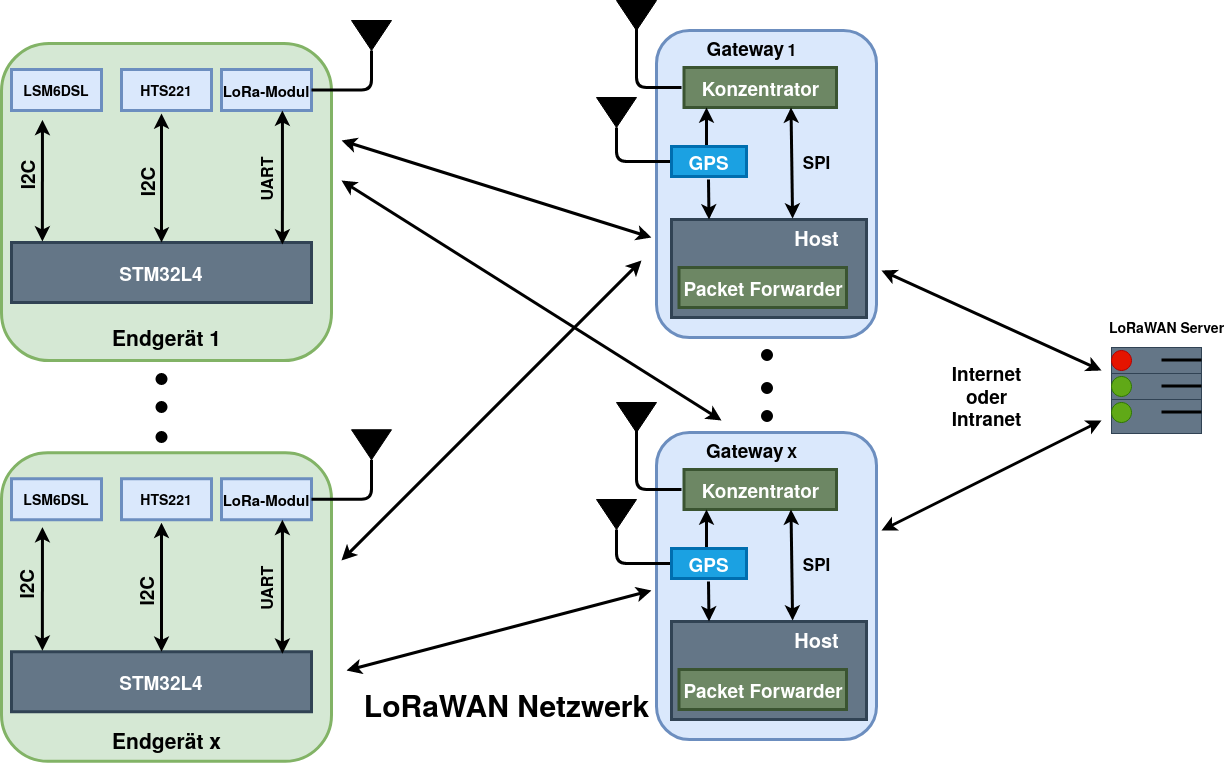
\includegraphics[width=15cm]{source/images/Gesamtsystem}
	\caption{Labcsmart IoT-Netzwerk \label{fig:LabcsmartLoRawan}}
\end{figure}


\begin{description}
	\newpage
	\item[LoRa:] ist eine Abk"urzung f"ur 
	\textbf{\textit{Long Range}} 
	und ist eine drahtlose Technologie, welche geringe 
	Sendeleistung 
	verbraucht, um kleine Datenpakete (0,3 \ac{Kbps} 
	bis 5,5 Kbps) "uber 
	eine lange Strecke zu senden oder zu empfangen.    
	
	\item[End Node Endger"at:] ist ein Ger"at, das aus 
	zwei Teilen 
	besteht, ein Funkmodul mit Antenne und ein 
	Mikrocontroller zur 
	Verarbeitung der Daten wie Sensordaten. Diese Daten 
	k"onnen entweder 
	an ein anderen LoRa-Endger"at per 
	Point-To-Point-Verbindung oder an 
	einen LoRaWAN-Server versandt werden.

	\item[LoRaWAN:] steht f"ur \textbf{\textit{Long 
	Range Wide Area 
	Network}} und ist das Kommunikationsprotokoll f"ur 
	das Netzwerk.
	
	\item[Gateway:] ist ein Ger"at, das aus mindestens 
	einem 
	Funkkonzentrator, einem Host und einer 
	Netzverbindung zum Internet 
	oder ein privates Netzwerk (Ethernet, 3G, Wi-Fi), 
	m"oglicherweise 
	einem \ac{GPS}-Empf"anger besteht.
	
	\item[LoRaWAN Server:] ist ein abstrakter Computer, 
	der die von dem 
	Gateway empfangene RF-Pakete verarbeitet und "ubersendet die 
	RF-Pakete als Antwort an das Gateway zur"uck.
	\vspace{1cm}
	\item[Application Server:] ist eine Anwendung, 
	womit der Benutzer 
	die von den Sensoren gemessenen Daten entweder 
    tabellarisch oder 
	grafisch auswerten kann.
	
	\item[Uplink:] ist die Kommunikation von einem 
	Endger"at zu einem 
	Gateway. 
	
	\item[Downlink:] ist die Kommunikation von einem 
	Gateway zu einem 
	Endger"at.
\end{description}


\section{Gliederung der Arbeit}

Das Kapitel \ref{Komponente} gibt einen detaillierten 
"Uberblick "uber allen Hardware-Komponen-ten, die bei 
der Entwicklung eines Endger"at verwendet werden. Als 
Erstes wird auf die Eigenschaften von dem benutzten 
STM32-Nucleo Board eingegangen. Diesem Kapitel ist auch 
zu entnehmen, warum genau dieses Board gew"ahlt wurde. 

Als n"achstes wird auf das LoRa-Modul eingegangen. 
Dieses LoRa-Modul 
wird dazu verwendet, um die erfassten Daten dem 
Server drahtlos zu "ubertragen. Dieses Kapitel 
berichtet "uber das Funkprotokol, das zur "Ubertragung 
der Daten eingesetzt wurde und wie diese Daten 
gesichert werden.
 
Das Kapitel \ref{G_S} beschreibt den LoRaWAN-Server und 
das Gateway, zwei wichtige Teile dieser Thesis. Die 
Funktionsweise wird erkl"art und die Servereinstellung 
wird gezeigt. Diese Einstellung sind notwendig, da
diese dem endger"at den Zutritt in das Netzwerk gew"ahren.

Als n"achstes wird die Softwareentwicklung behandelt. 
Hier geht es zu Beginn um die Entwicklungsumgebung des 
gesamten Projekts (Eclipse).Anschlie\ss{}end daran 
werden die angewandten Bibliotheken dargestellt, 
ihre Installation und Nutzung erkl"art. Es wurde f"ur 
diese Arbeit zwei bekannte Kommunikationsschnittstellen 
verwendet (\ac{I2C} und \ac{UART}). Sie erfahren ebenfalls wie diese 
Schnittstellen mit der Programmiersprache-C angesteuert 
werden und welche Software-Tricks eingesetzt wurden, 
um AT-Befehle zu senden.

Anschlie\ss{}end  wird im Kapitel \ref{Fazit} eine 
Zusammenfassung und eine kleine Ausblick der Arbeit 
gegeben.
   